\documentclass[11pt,letterpaper]{article}
\PassOptionsToPackage{hyphens}{url}
\usepackage[margin=.83in,top=.8in,bottom=.8in,headheight=15pt]{geometry}
\usepackage[T1]{fontenc}
\usepackage{lmodern,amsmath,amssymb,mathtools,bm,booktabs,array,graphicx,tikz}
\usetikzlibrary{arrows.meta,positioning,calc,decorations.pathreplacing,patterns}
\definecolor{ink}{HTML}{17344D}\definecolor{accent}{HTML}{087E8B}\definecolor{pale}{HTML}{EDF5F5}\definecolor{gold}{HTML}{AD6B19}
\providecommand{\dd}{\,\mathrm{d}}\providecommand{\R}{\mathbb{R}}
\providecommand{\E}{\mathbb{E}}\providecommand{\Var}{\operatorname{Var}}
\providecommand{\Cov}{\operatorname{Cov}}\providecommand{\diag}{\operatorname{diag}}
\providecommand{\norm}[1]{\left\lVert#1\right\rVert}
\providecommand{\abs}[1]{\left|#1\right|}
\usepackage{microtype,hyperref,fancyhdr,enumitem,amsthm,sectsty,needspace}
\allsectionsfont{\raggedright}
\hypersetup{colorlinks=true,linkcolor=ink,urlcolor=accent,pdfauthor={Zan Ahmad},pdftitle={Coordinates, sampled motion, and Python expressions / Lecture notes}}
\setlength{\parindent}{0pt}\setlength{\parskip}{6pt}\linespread{1.07}
\setlist{itemsep=3pt,topsep=4pt,leftmargin=*}
\emergencystretch=2em\clubpenalty=10000\widowpenalty=10000
\pagestyle{fancy}\fancyhf{}\fancyhead[L]{\small Scientific Computing in Python / 2027}\fancyhead[R]{\small Lecture 1}
\fancyfoot[L]{\footnotesize Zan Ahmad}\fancyfoot[R]{\footnotesize\thepage}\renewcommand{\headrulewidth}{.3pt}
\newtheorem{proposition}{Proposition}\newtheorem{theorem}{Theorem}\newtheorem{lemma}{Lemma}
\theoremstyle{definition}\newtheorem{definition}{Definition}\newtheorem{example}{Example}
\numberwithin{equation}{section}
\begin{document}
{\small\scshape Scientific Computing in Python / 2027\hfill Lecture 1}\par\medskip
{\raggedright\hyphenpenalty=10000\exhyphenpenalty=10000\LARGE\bfseries\color{ink} Coordinates, sampled motion, and Python expressions\par}\medskip
{\small Lecture notes}\par\bigskip
Two objects are observed at the same times. One finishes farther along the ruler, while the other moves farther during the observation interval. We shall express both comparisons precisely, translate them into Python, and examine which statements are unchanged by a change of origin or unit. These elementary invariances will later become useful tests of larger numerical programs.

\section{Position and displacement}
\hypertarget{note-position-and-displacement}{}\label{note:position-and-displacement}
{\small \href{slides.html\#frame=position-and-displacement\&step=1}{Slides for this section}}\par
Let $x_i$ be a position measured from a specified origin at time $t_i$. Position depends on that origin. Displacement is a difference of positions and describes the change over a stated interval. The synthetic records use millimeters and seconds. Their regularly spaced points describe observations; a continuous trajectory between them is an additional assumption.

\[
t=(0,2,4,6,8),\quad x_A=(10,14,18,22,26),\quad x_B=(0,6,12,18,24).
\]

At $t=8$, $x_A>x_B$, but $\Delta x_A=16<24=\Delta x_B$.

\subsection*{Average velocities}
\[
\overline v_A=\frac{26-10}{8-0}=2\ \mathrm{mm/s},\qquad
\overline v_B=\frac{24-0}{8-0}=3\ \mathrm{mm/s}.
\]

Final position and average velocity answer different comparisons.
\section{Assignment and evaluation}
\hypertarget{note-assignment-and-evaluation}{}\label{note:assignment-and-evaluation}
{\small \href{slides.html\#frame=assignment-and-evaluation\&step=1}{Slides for this section}}\par
Python evaluates the right-hand side of an assignment and stores a reference to its result. Changing one input afterward does not automatically recompute earlier expressions. In a notebook, execution order determines the state. A clean restart followed by execution in order provides a reproducible sequence of assignments.

\begin{minipage}{\linewidth}
\begin{verbatim}
a_mm = [10, 14, 18, 22, 26]
displacement = a_mm[-1] - a_mm[0]
elapsed = 8 - 0
velocity = displacement / elapsed
\end{verbatim}
\end{minipage}

\Needspace{8\baselineskip}\subsection*{Reassignment}
\begin{minipage}{\linewidth}
\begin{verbatim}
a = 10
b = a + 2
a = 20
\end{verbatim}
\end{minipage}

The final values are $a=20$ and $b=12$. Python has executed statements, not solved simultaneous equations.
\section{Translation of the coordinate origin}
\hypertarget{note-translation-of-the-coordinate-origin}{}\label{note:translation-of-the-coordinate-origin}
{\small \href{slides.html\#frame=translation-of-the-coordinate-origin\&step=1}{Slides for this section}}\par
Choose a new origin by replacing every position by $x_i'=x_i+c$, with the same constant $c$. The displacement is unchanged because the offset cancels. A change of time origin also leaves elapsed times unchanged. Thus the average velocity depends on the separation of coordinates rather than their arbitrary zero points.

\[
\Delta x'=(x_1+c)-(x_0+c)=x_1-x_0=\Delta x.
\]

\[
\frac{\Delta x'}{(t_1+d)-(t_0+d)}=\frac{\Delta x}{\Delta t}.
\]

\subsection*{An invariance test}
\begin{minipage}{\linewidth}
\begin{verbatim}
shifted = (26 + 100) - (10 + 100)
assert shifted == 26 - 10
\end{verbatim}
\end{minipage}

A failed test indicates that the code depends on the origin in a way that the defined statistic does not.
\begin{center}\begin{minipage}{.98\linewidth}\centering
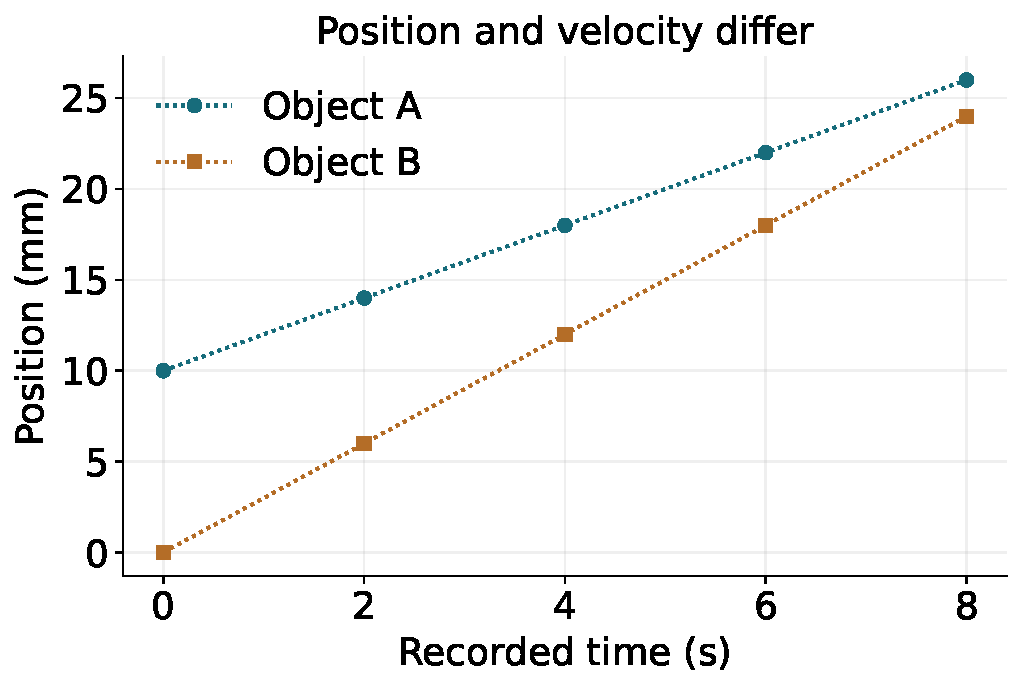
\includegraphics[width=.96\linewidth,height=.57\textheight,keepaspectratio]{position-records.pdf}\par\smallskip
{\small Synthetic position observations in a shared ruler coordinate; dotted connectors are visual guides, not a fitted motion law.}
\end{minipage}\end{center}
\section{Change of physical units}
\hypertarget{note-change-of-physical-units}{}\label{note:change-of-physical-units}
{\small \href{slides.html\#frame=change-of-physical-units\&step=1}{Slides for this section}}\par
If position is rescaled by a factor $a$ and time by a factor $b$, the numerical velocity is rescaled by $a/b$. This is a transformation law, not invariance of the numerical value. Millimeters to centimeters uses $a=1/10$. Seconds to minutes uses $b=1/60$. Keeping the numerical value while changing the printed unit would change the physical quantity.

\[
x'=ax,\quad t'=bt\quad\Longrightarrow\quad\overline v'=\frac ab\overline v.
\]

\[
2\ \mathrm{mm/s}=0.2\ \mathrm{cm/s}=12\ \mathrm{cm/min}.
\]

\subsection*{Numerical comparison after conversion}
\begin{minipage}{\linewidth}
\begin{verbatim}
dx_mm = 26 - 10
dx_cm = 26/10 - 10/10
assert abs(10*dx_cm - dx_mm) < 1e-12
\end{verbatim}
\end{minipage}

The tolerance accounts for rounding, not measurement uncertainty.
\section{Displacement and path length}
\hypertarget{note-displacement-and-path-length}{}\label{note:displacement-and-path-length}
{\small \href{slides.html\#frame=displacement-and-path-length\&step=1}{Slides for this section}}\par
In one dimension the endpoint displacement may vanish even when substantial motion occurred. Summing absolute increments yields the length of the polygonal path through the samples. The triangle inequality shows that this sampled length is at least the magnitude of endpoint displacement. Unobserved motion can make the actual path longer still.

\[
\Delta x=x_N-x_0=\sum_{i=0}^{N-1}(x_{i+1}-x_i).
\]

\[
|\Delta x|\leq\sum_{i=0}^{N-1}|x_{i+1}-x_i|=L_{\rm sampled}.
\]

\subsection*{An out-and-back record}
For positions $0,4,0$ at times $0,1,2$,
\[
\Delta x=0,\qquad L_{\rm sampled}=8.
\]

The signed average velocity is zero. The sampled mean speed is $4$ distance units per time unit.
\begin{center}\begin{minipage}{.98\linewidth}\centering
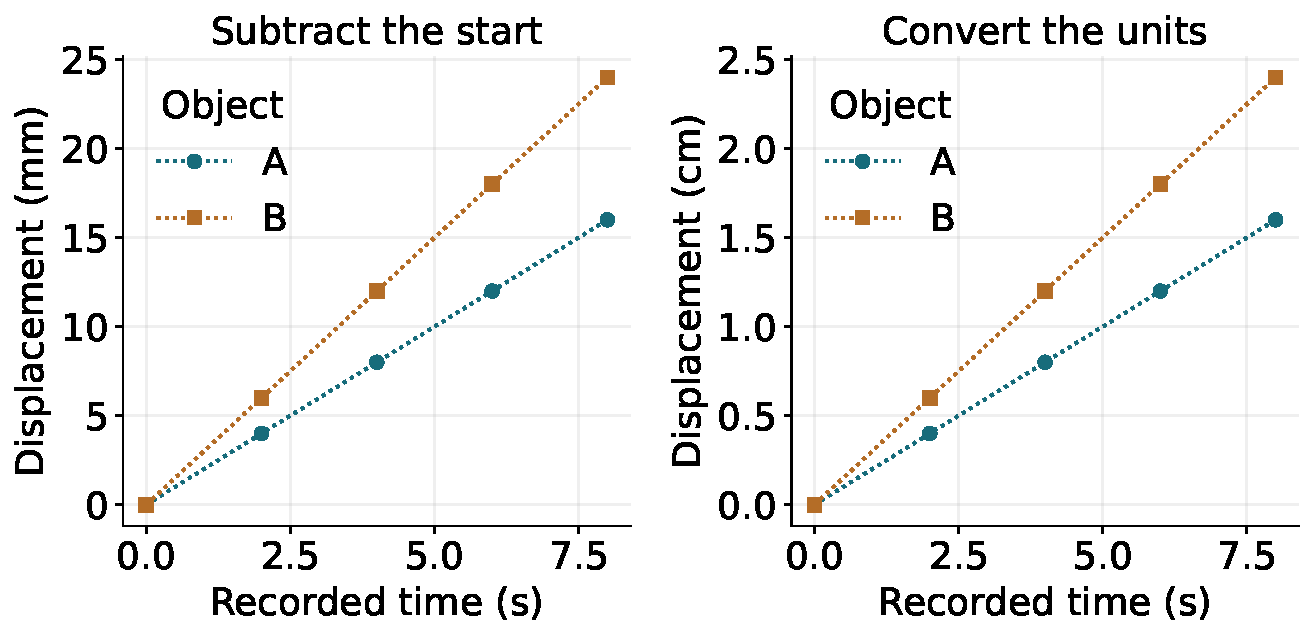
\includegraphics[width=.96\linewidth,height=.57\textheight,keepaspectratio]{displacement-units.pdf}\par\smallskip
{\small Both records are shown relative to their own starting positions, first in millimeters and then centimeters. The panels are unit conversions of the same data.}
\end{minipage}\end{center}
\Needspace{10\baselineskip}
\section{Information between samples}
\hypertarget{note-information-between-samples}{}\label{note:information-between-samples}
{\small \href{slides.html\#frame=information-between-samples\&step=1}{Slides for this section}}\par
A plotted line connects observations but does not establish constant velocity between them. Changing an interior observation can change the sampled path length while leaving endpoint displacement unchanged. The supplied notebook separates baseline figures from an editable plotting cell, so that a changed record can be displayed explicitly.

Two trajectories can agree at every sample time while differing between them.

For a smooth interpolant $x(t)$, add
\[
g(t)=c\prod_i(t-t_i).
\]
The sampled positions stay fixed.

\subsection*{Array order and data correspondence}
\begin{minipage}{\linewidth}
\begin{verbatim}
assert len(times_s) == len(a_mm)
plt.plot(times_s, a_mm, "o")
\end{verbatim}
\end{minipage}

The $i$th time and $i$th position must belong to the same observation. Equal lengths alone do not prove correct pairing.
\bigskip
\section*{Exercises}
\par\noindent\begin{minipage}{\linewidth}
\subsection*{P27-1-1. Choose the quantity}
A new synthetic record starts at 7 mm and ends at 19 mm over 6 s. Total: 10 formative points.

\textbf{a} Calculate displacement and interval-average velocity with units.

\end{minipage}\par\medskip
\textbf{b} A program uses 19/6. What question does this fail to answer, and why?

\textbf{c} Could the object have reversed direction between observations? What would that change about a speed claim?

\par\noindent\begin{minipage}{\linewidth}
\subsection*{P27-1-2. Execution and types}
Assume x0=\allowbreak{}3, x1=\allowbreak{}15, elapsed=\allowbreak{}4; displacement is assigned x1-x0 before x1 changes to 23. Total: 10 points.

\textbf{a} State the stored displacement before and after its assignment is rerun.

\end{minipage}\par\medskip
\textbf{b} State the corresponding average velocity after each displacement calculation, if positions are mm and time is s.

\textbf{c} Explain how the text "23" differs from the number 23, and give a reproducibility check.

\par\noindent\begin{minipage}{\linewidth}
\subsection*{P27-1-3. Two transformations}
A position record is [-2,4,10] mm at [0,3,6] s. Total: 10 points.

\textbf{a} Calculate displacement and signed average velocity.

\end{minipage}\par\medskip
\textbf{b} Add 100 mm to each coordinate and recalculate the displacement. Explain the result.

\textbf{c} Convert the original coordinates and average velocity to centimeters and centimeters per second. Give a reverse check.

\par\noindent\begin{minipage}{\linewidth}
\subsection*{P27-1-4. An honest graphical record}
A plot connects three position observations with smooth curves. Total: 10 points.

\textbf{a} Name the two required axis quantities and units for a record stored in seconds and millimeters.

\end{minipage}\par\medskip
\textbf{b} Explain two checks that preserve pairing and usable time intervals.

\textbf{c} Write a defensible caption that distinguishes samples from the curves.

\section*{References}
\noindent\begin{minipage}{\linewidth}
Original Python Lecture 0. PDF pages 15--21 and 38--43.

\url{https://zanahmad.com/files/scientific-python/Lecture_0__Intro_to_Python.pdf}
\end{minipage}\par\medskip
Python source materials: Phillip Kerger (2023). Course adaptation and additional exposition: Zan Ahmad.

\end{document}
